\chapter{RESULTADOS DE SIMULAÇÕES}
\label{resultados}
\section{\textbf{Introdução}}
Neste capítulo serão apresentadas as simulações realizadas para analisar o comportamento de partículas presentes em turbomáquinas em ação.
Foram escolhidos quatro tipos de geometria para serem simulados:
\begin{itemize}
    \item \textbf{Canal reto}.

        Uma geometria simples, que busca simular o comportamento básico das partículas sobre efeito de um escoamento. 
        A malha utilizada tem $1072$ elementos definidos sobre $593$ nós, exposta na \ref{channel_mesh}.
        \begin{figure}[H]
            \centering
            \stackunder{
                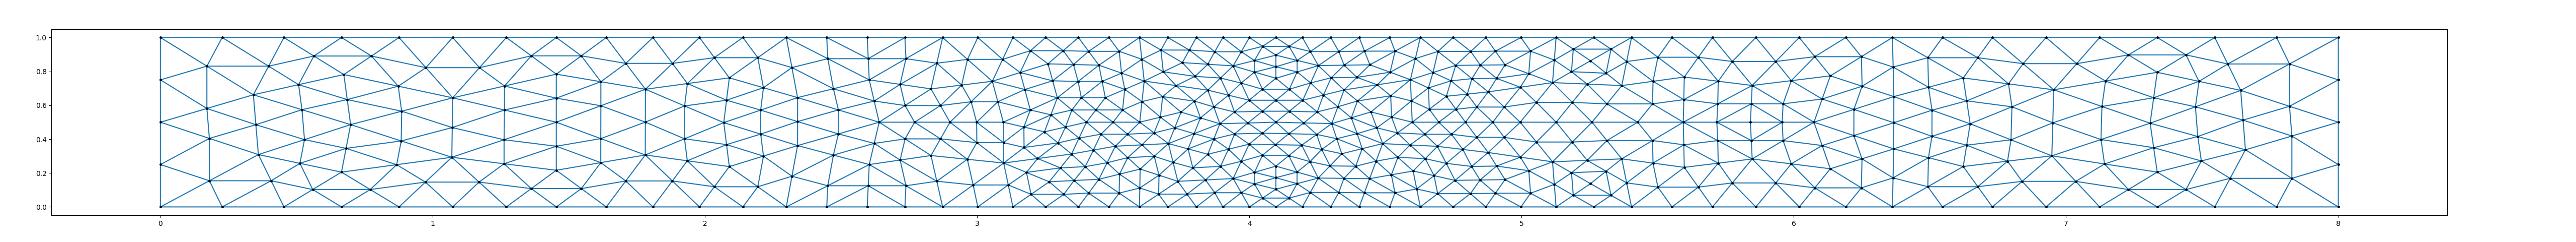
\includegraphics[width=\linewidth]{figures/Channel_mesh.png}
            } {\raggedleft \scriptsize Fonte: Autor.}
            \caption{Malha da simulação em um canal reto.}
            \label{channel_mesh}
        \end{figure}

    \item \textbf{Canal com um obstáculo circular no centro}.

        Esta geometria visa simular o efeito de obstáculos, ou até mesmo as próprias partículas no escoamento.
        Porém, não é utilizada neste trabalho a implementação \textit{two-way}, que levaria em conta os efeitos das partículas no escoamento.
        Neste caso a simulação foi aplicada a uma malha de $868$ elementos e $494$ nós.
        \begin{figure}[H]
            \centering
            \stackunder{
                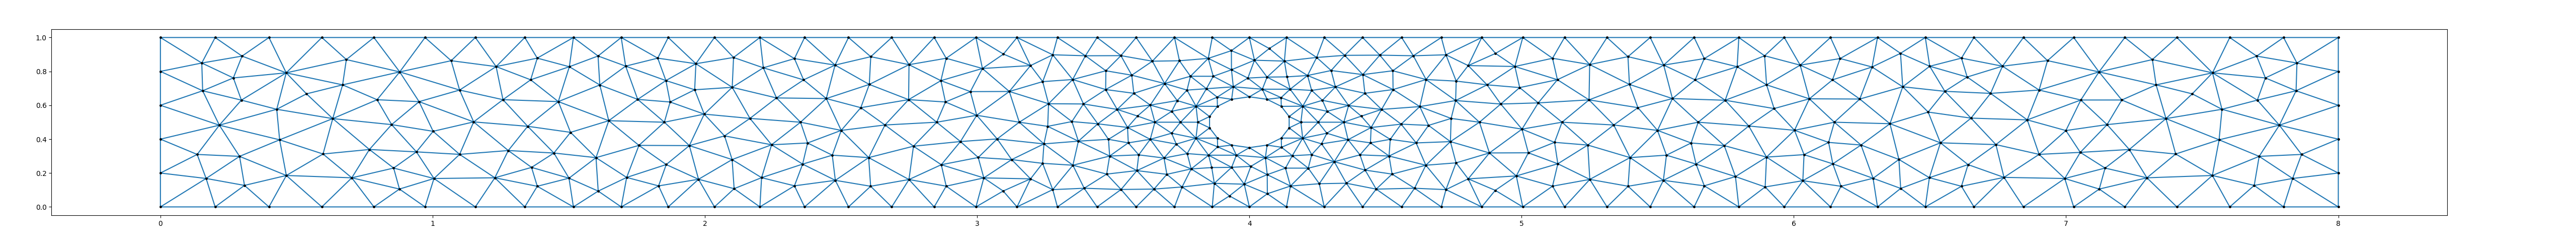
\includegraphics[width=\linewidth]{figures/Obstacle_mesh.png}
            } {\raggedleft \scriptsize Fonte: Autor.}
            \caption{Malha da simulação em um canal com um obstáculo.}
            \label{obstacle_mesh}
        \end{figure}

    \item \textbf{Canal com degrau}.

        O escoamento em um canal com um degrau, ou uma diferença brusca de percurso em seu trajeto, possui diversos efeitos interessantes de se observar.
        Como por exemplo as regiões 
        Com uma malha de $676$ elementos definidos sobre $380$ nós.
        \begin{figure}[H]
            \centering
            \stackunder{
                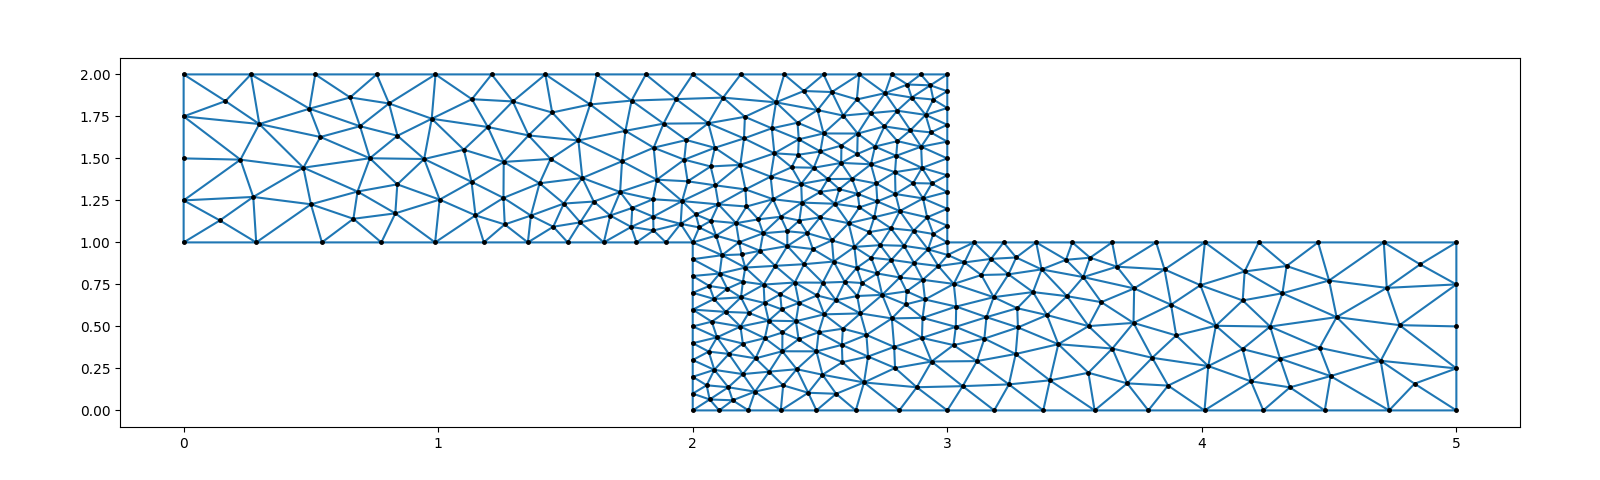
\includegraphics[width=\linewidth]{figures/Step_mesh.png}
            } {\raggedleft \scriptsize Fonte: Autor.}
            \caption{Malha da simulação em um canal com degrau.}
            \label{step_mesh}
        \end{figure}

    \item \textbf{Pá de um rotor}.

        Finalmente, será analizado o comportamento de partículas em um escoamento presente em uma seção de um rotor de uma turbomáquina.
        Neste trabalho, foi tomado um referencial estacionário na pá, sem efeito da rotação do rotor no escoamento.
        Foi utilizada uma malha de $1058$ elementos definidos sobre $531$ nós.
        \begin{figure}[H]
            \centering
            \stackunder{
                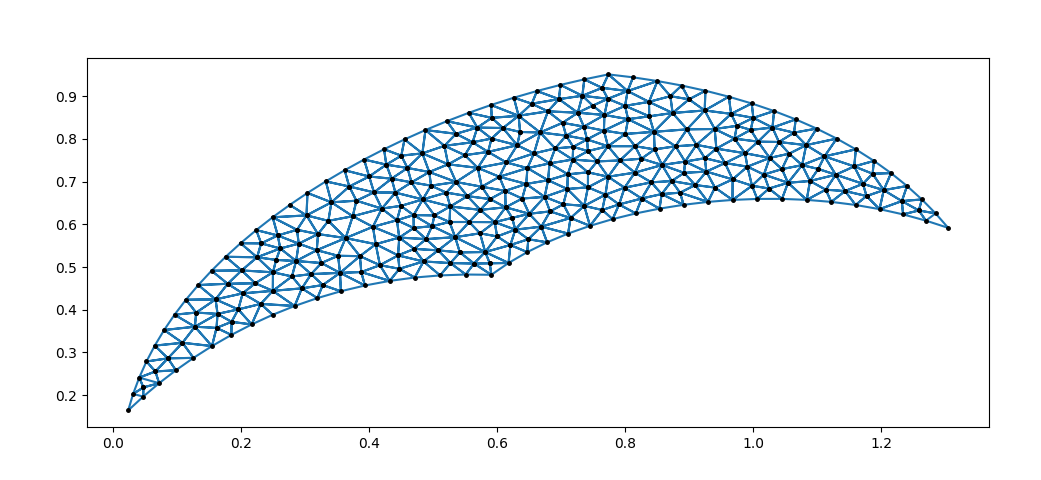
\includegraphics[width=\linewidth]{figures/Rotor_mesh.png}
            } {\raggedleft \scriptsize Fonte: Autor.}
            \caption{Malha da simulação em uma pá de um rotor.}
            \label{rotor_mesh}
        \end{figure}
\end{itemize}
